\documentclass{article}
\usepackage{amsmath, sfmath, multicol, tkz-euclide, array, enumerate, tcolorbox, tabularray, tipa}
\renewcommand{\familydefault}{\sfdefault}
\setlength{\parindent}{0cm}
\pagestyle{empty}
\usepackage[left=1in, top=0.5in, right=1in, bottom=0.5in]{geometry}
\tikzset{>=stealth, label style/.append style={font=\footnotesize}}
\tcbset{colback=white}

\newcounter{example}[section]
\newenvironment{example}[1][]{\refstepcounter{example}\par\medskip
   {\color{red}\textbf{Example~\theexample. #1}}}{\medskip}

\newcommand{\arc}[1]{%
    \setbox9=\hbox{#1}%
    \ooalign{\resizebox{\wd9}{\height}{\texttoptiebar{\phantom{A}}}\cr#1}}

\begin{document}

\section*{Circles and Arcs}

\begin{tcolorbox}[colframe=orange!70!white, coltitle=black, title=\textbf{Today I Can}]
\begin{enumerate}
    \item Find the measures of central angles and arcs.
    \item Find arc length.
\end{enumerate}
\end{tcolorbox}
\smallskip 

\begin{tcolorbox}[colframe=black!20!white, opacitybacktitle=0.1, coltitle=black, title=\textbf{Circle Properties}]
\begin{minipage}{0.5\textwidth}
    \begin{itemize}
        \item $P$ is the center of the circle.
        \item $\overline{PC}$ is a radius.
        \item $\overline{AB}$ is a diameter.
        \item $\angle APC$ is a \textbf{central angle}.
    \end{itemize}
\end{minipage}
\begin{minipage}{0.4\textwidth}
    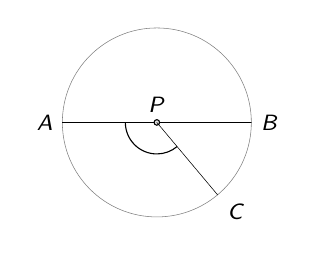
\begin{tikzpicture}[scale=0.8]
    \tkzDefPoints{0/0/P, -1.5/0/A, 1.5/0/B}
    \tkzDrawCircle(P,A)
    \tkzDrawSegment(A,B)
    \tkzDrawPoint(P)
    \tkzLabelPoints[left](A)
    \tkzLabelPoints[above](P)
    \tkzLabelPoints[right](B)
    \tkzDefShiftPoint[P](-50:1.5){C}
    \tkzDrawSegment(P,C)
    \tkzLabelPoints[below right](C)
    \tkzMarkAngle[size=.5](A,P,C)
\end{tikzpicture}
\end{minipage}
\end{tcolorbox}
\bigskip 

\setlength{\extrarowheight}{5pt}
\begin{tabular}{|c|c|c|}
\hline
\textbf{Term}   &   \textbf{Definition} &   \textbf{Diagram}    \\[3pt] \hline
Circle  &   Set of all points equidistant from a given point (the \emph{center}) &
$\odot P$   \\[3pt] \hline
Diamter &   Segment through the center with endpoints on the circle &   $\overline{AB}$ \\[3pt] \hline
Radius  &   Segment connecting center and the edge  &  $\overline{PA}$, $\overline{PB}$, $\overline{PC}$ \\[3pt] \hline
Congruent Circles   &   Circles with congruent radii   &   \\[3pt] \hline
Central Angle   &   Angle with vertex as circle's center &   $\angle APC \text{ and } \angle BPC$ \\[3pt] \hline  
Minor Arc   &   Part of the circle less than half of it  &   $\arc{\textit{AC}} \text{ and } \arc{\textit{BC}}$  \\[3pt] \hline
Semi Circle &   Half the circle &   $\arc{\textit{ACB}}$    \\[3pt] \hline
Major Arc   &   Part of the circle more than half of it  &   $\arc{\textit{ABC}}$    \\[3pt] \hline
\end{tabular}
\bigskip  

\begin{example}
Answer each of the following given $\odot O$. \newline 

\begin{minipage}{0.3\textwidth}
    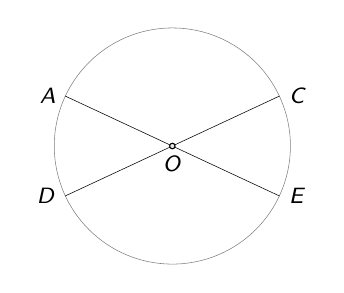
\begin{tikzpicture}
    \tkzDefPoints{0/0/O}
    \tkzDefShiftPoint[O](25:1.5){C}
    \tkzDefShiftPoint[O](155:1.5){A}
    \tkzDefShiftPoint[O](205:1.5){D}
    \tkzDefShiftPoint[O](-25:1.5){E}
    \tkzDrawCircle(O,C)
    \tkzDrawSegments(A,E D,C)
    \tkzLabelPoints[left](A,D)
    \tkzLabelPoints[right](E,C)
    \tkzLabelPoints[below](O)
    \tkzDrawPoint(O)
    \end{tikzpicture}
\end{minipage}
\begin{minipage}{0.5\textwidth}
    \begin{enumerate}[(a)]  \setlength{\itemsep}{25pt}
        \item What are the minor arcs of $\odot O$? 
        \item What are the semi circles of $\odot O$?
        \item What are the major arcs of $\odot O$?
    \end{enumerate}
\end{minipage}
\end{example}
\vspace{0.35in}

\begin{tcolorbox}[colframe=black!20!white, opacitybacktitle=0.1, coltitle=black, title=\textbf{Arc Measure}]
The measure of an arc is equal to the measure of its corresponding central angle.
\end{tcolorbox}

\begin{tcolorbox}[colframe=black!20!white, opacitybacktitle=0.1, coltitle=black, title=\textbf{Adjacent Arcs}]
Arcs on the same circle with one common endpoint.
\end{tcolorbox}

\begin{tcolorbox}[colframe=black!20!white, opacitybacktitle=0.1, coltitle=black, title=\textbf{Arc Addition Postulate}]
\begin{minipage}{0.4\textwidth}
    \begin{itemize}
        \item $m\arc{\textit{ABC}} = m\arc{\textit{AB}} + m\arc{\textit{BC}}$
    \end{itemize}
\end{minipage}
\begin{minipage}{0.4\textwidth}
    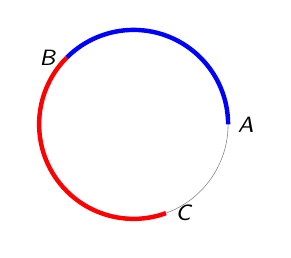
\begin{tikzpicture}[scale=0.8]
    \tkzDefPoints{0/0/O, 1.5/0/A}
    \tkzDefShiftPoint[O](135:1.5){B}
    \tkzDefShiftPoint[O](290:1.5){C}
    \tkzDrawCircle(O,A)
    \tkzLabelPoints[right](A,C)
    \tkzLabelPoints[left](B)
    \draw [ultra thick, color=blue] (A) arc (0:135:1.5);
    \draw [ultra thick, color=red] (B) arc (135:290:1.5);
    \end{tikzpicture}
\end{minipage}
\end{tcolorbox}
\bigskip 

\begin{example}
What is the measure of each arc in $\odot O$?   \newline 

\begin{minipage}{0.4\textwidth}
    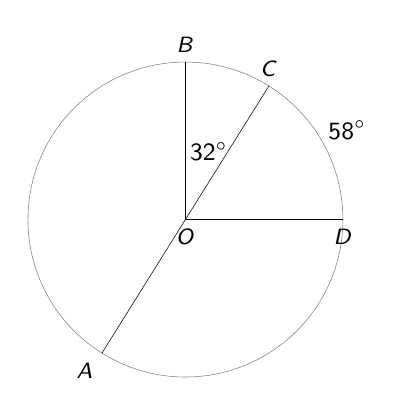
\begin{tikzpicture}
    \tkzDefPoints{0/0/O, 2/0/D}
    \tkzDefShiftPoint[O](58:2){C}
    \tkzDefShiftPoint[O](90:2){B}
    \tkzDefShiftPoint[O](238:2){A}
    \tkzDrawCircle(O,D)
    \tkzDrawSegments(O,A O,B O,C O,D)
    \tkzLabelPoints[above](B,C)
    \tkzLabelPoints[](D,O)
    \tkzLabelPoints[below left](A)
    \tkzLabelAngle[pos=2.35](D,O,C){\small $58^\circ$}
    \tkzLabelAngle[pos=0.9,xshift=0.05cm](C,O,B){\small $32^\circ$}
    \end{tikzpicture}
\end{minipage}
\begin{minipage}{0.4\textwidth}
    \begin{enumerate}[(a)]  \setlength{\itemsep}{20pt}
       \item $\arc{\textit{BC}}$
        \item $\arc{\textit{BD}}$
        \item $\arc{\textit{ABC}}$
        \item $\arc{\textit{AB}}$ 
    \end{enumerate}
\end{minipage}
\end{example}
\bigskip 

\begin{tcolorbox}[colframe=black!20!white, opacitybacktitle=0.1, coltitle=black, title=\textbf{Arc Length}]
A fraction of the circle's circumference. \newline 

\begin{minipage}{0.4\textwidth}
    \begin{itemize}
        \item Length of $\arc{\textit{AB}} = \dfrac{m\arc{\textit{AB}}}{360^\circ} \cdot 2\pi r$
    \end{itemize}
\end{minipage}
\begin{minipage}{0.4\textwidth}
    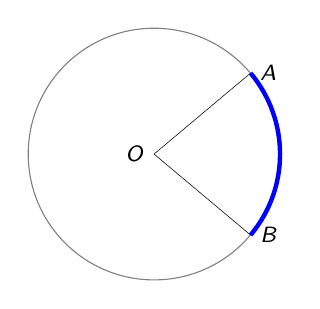
\begin{tikzpicture}[scale=0.8]
    \tkzDefPoints{0/0/O}
    \tkzDefShiftPoint[O](40:2){A}
    \tkzDefShiftPoint[O](-40:2){B}
    \tkzDrawCircle[thin](O,A)
    \tkzDrawSegments(O,A O,B)
    \tkzLabelPoints[right](A,B)
    \tkzLabelPoints[left](O)
    \draw [ultra thick, color=blue] (B) arc (-40:40:2);
    \end{tikzpicture}
\end{minipage}
\end{tcolorbox}
\bigskip 

\begin{example}
Find the length of each arc.
\begin{enumerate}[(a)]
    \begin{multicols}{2}
    \item $\arc{\textit{XY}}$
    \item $\arc{\textit{XPY}}$
    \end{multicols}
\end{enumerate}
\begin{minipage}{0.5\textwidth}
    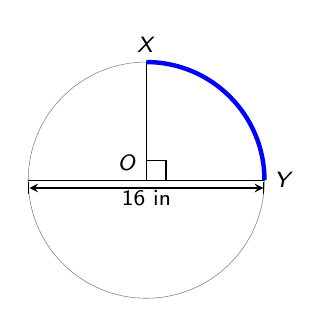
\begin{tikzpicture}
    \tkzDefPoints{0/0/O, 1.5/0/Y, 0/1.5/X, -1.5/0/Z}
    \tkzDrawCircle(O,X)
    \tkzMarkRightAngle(Y,O,X)
    \tkzDrawSegments(O,Y O,X O,Z)
    \tkzLabelSegment[below,yshift=-0.01cm](Y,Z){16 in}
    \draw[|<->|, >=stealth, yshift=-0.1cm] (-1.5,0) -- (1.5,0);
    \draw[ultra thick, color=blue] (1.5,0) arc (0:90:1.5);
    \tkzLabelPoints[above](X)
    \tkzLabelPoints[right](Y)
    \tkzLabelPoints[above left](O)
    \end{tikzpicture}
\end{minipage}
\begin{minipage}{0.4\textwidth}
    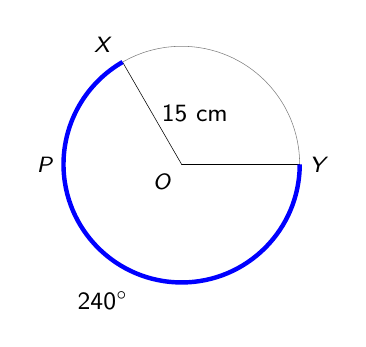
\begin{tikzpicture}
    \tkzDefPoints{0/0/O, 1.5/0/Y, -1.5/0/P}
    \tkzDefShiftPoint[O](120:1.5){X}
    \tkzDrawCircle(O,X)
    \tkzDrawSegments(O,Y O,X)
    \tkzLabelPoints[right](Y)
    \tkzLabelPoints[below left](O)
    \tkzLabelPoints[left](P)
    \tkzLabelPoints[above left](X)
    \tkzLabelSegment[right](X,O){\small 15 cm}
    \tkzLabelAngle[pos=-2](Y,O,X){\small $240^\circ$}
    \draw [ultra thick, color=blue] (1.5,0) arc (0:-240:1.5);
    \end{tikzpicture}
\end{minipage}
\end{example}

\end{document}
